% !TeX root = ../main.tex

\appendix{B}{系統UML圖}
本附錄包含了自主身分(AID)系統的各種UML圖表,旨在從不同角度展示系統的結構、流程和交互。這些圖表有助於讀者更深入地理解AID系統的設計和運作機制。
\section{物件圖}
\begin{figure}
  \centering
  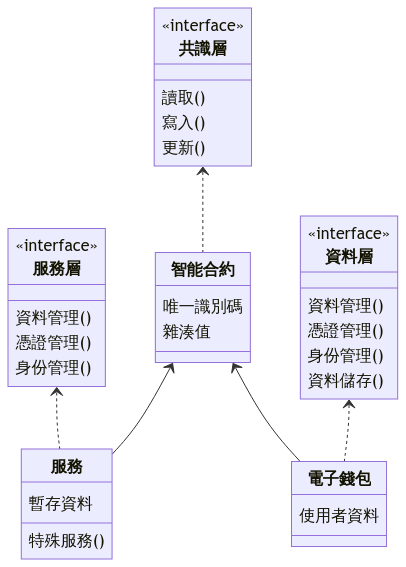
\includegraphics[width=\linewidth]{figures/design-struct.png}
  \caption{AID系統物件圖}
  \label{fig:appendix-aid-struct}
\end{figure}
物件圖展示了AID系統中各主要組件之間的靜態關係,有助於理解系統的整體架構。圖 \ref{fig:appendix-aid-struct} 呈現了AID系統的主要組件及其關係,包括共識層、服務層和數據層,以及它們之間的交互。
\section{時序圖}
時序圖展示了AID系統中各種重要流程的時間順序和組件間的交互,幫助讀者理解系統的動態行為。
\begin{itemize}
  \item 圖 \ref{fig:appendix-ca-uml} 展示了基本自主憑證的創建和使用流程,說明了用戶如何生成和管理自己的身份憑證。
  \item 圖 \ref{fig:appendix-da-uml} 描述了數據憑證的生成和驗證過程,展示了如何確保數據的真實性和可信度。
  \item 圖 \ref{fig:appendix-self-auth} 詳細說明了自主身分驗證的步驟,展示了用戶如何證明自己的身份。
  \item 圖 \ref{fig:appendix-full-aid-auth} 追加了第三方機構等額外功能的自主驗證流程,揭露更複雜場景的解決方案。
  \item 圖 \ref{fig:appendix-credit-uml} 展示了信用評分的計算和使用流程,說明了系統如何建立和維護用戶的信用。
\end{itemize}
\begin{figure}[p]
  \centering
  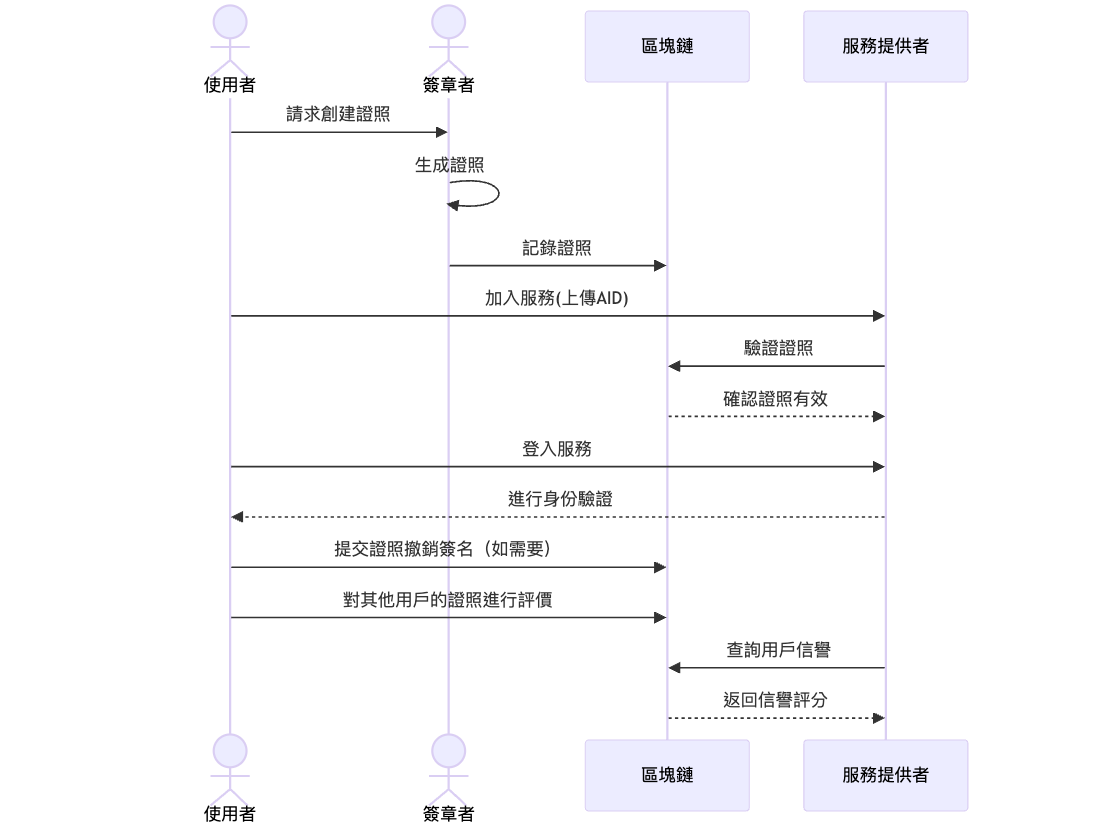
\includegraphics[width=\linewidth]{figures/CA-UML.png}
  \caption{自主憑證流程}
  \label{fig:appendix-ca-uml}
\end{figure}
\clearpage
\begin{figure}[p]
  \centering
  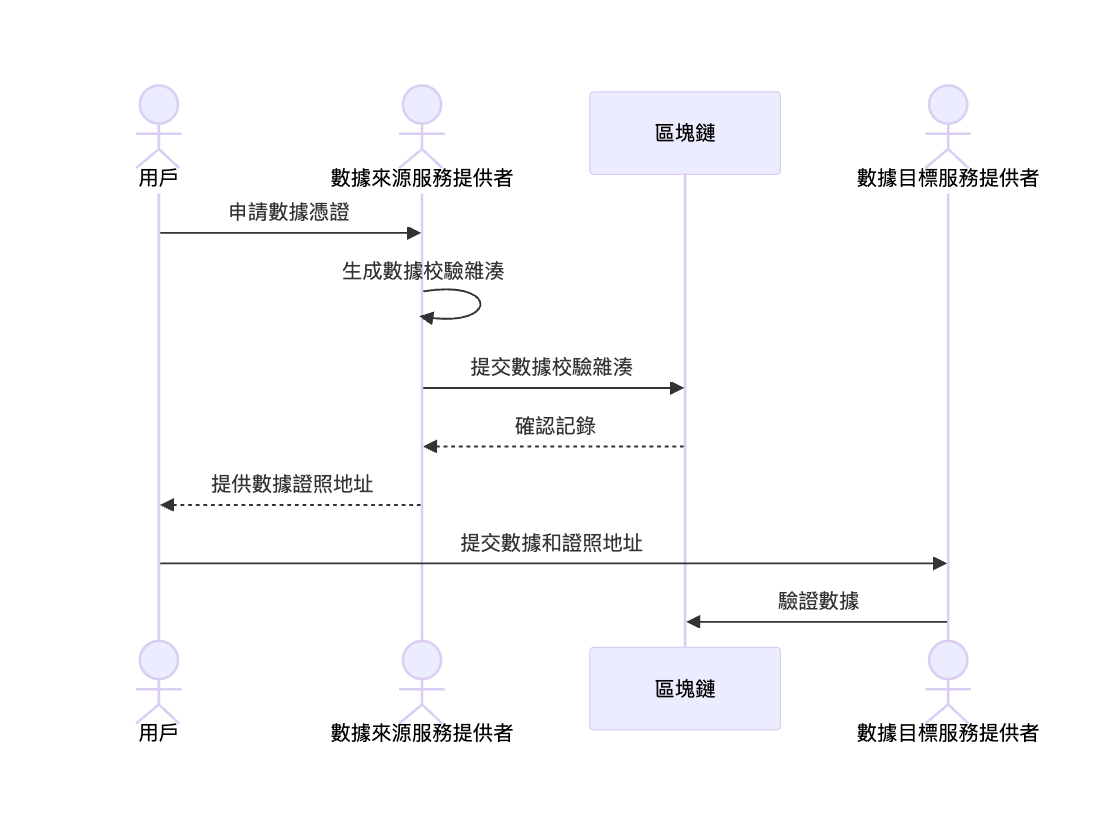
\includegraphics[width=\linewidth]{figures/DA-UML.png}
  \caption{數據憑證流程}
  \label{fig:appendix-da-uml}
\end{figure}
\clearpage
\begin{figure}[p]
  \centering
  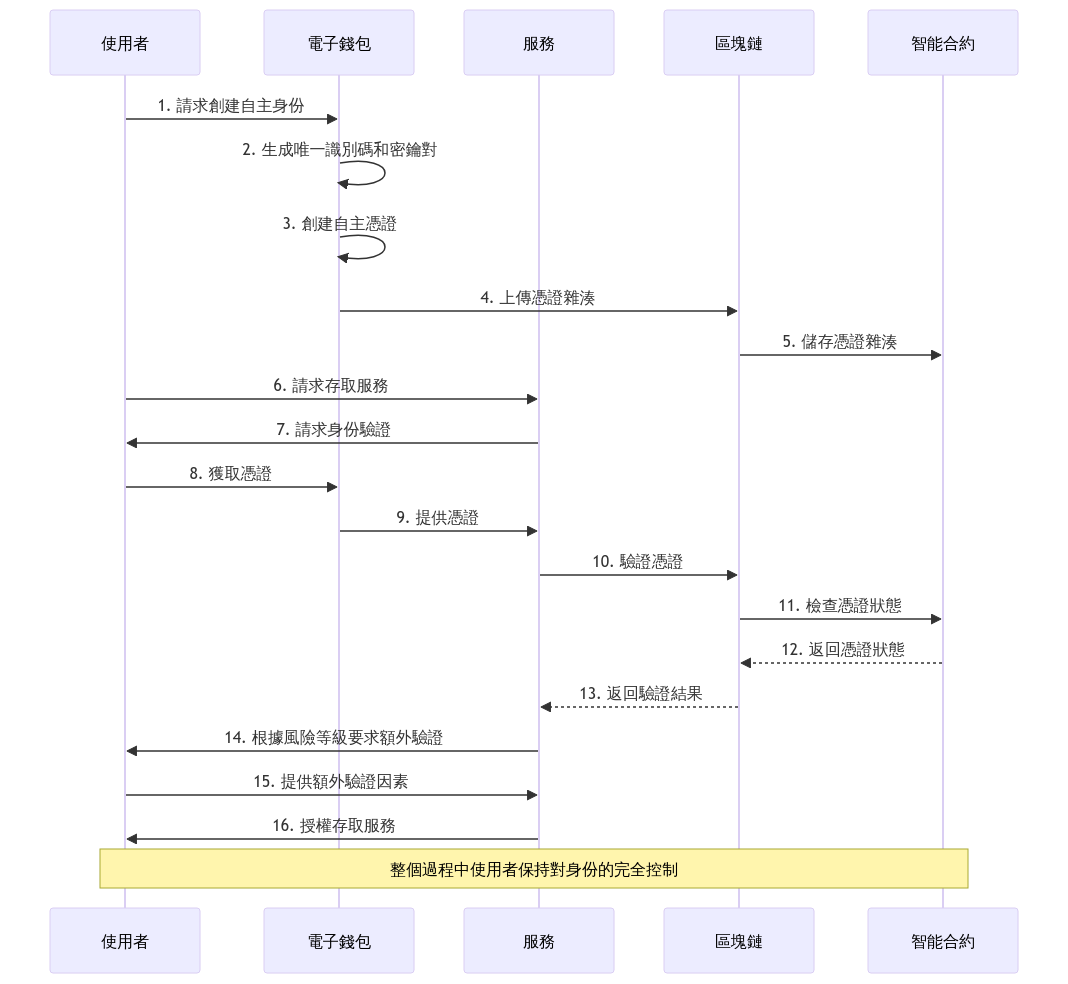
\includegraphics[width=\linewidth]{figures/new-self-auth.png}
  \caption{自主身分驗證流程}
  \label{fig:appendix-self-auth}
\end{figure}
\clearpage
\begin{figure}[p]
  \centering
  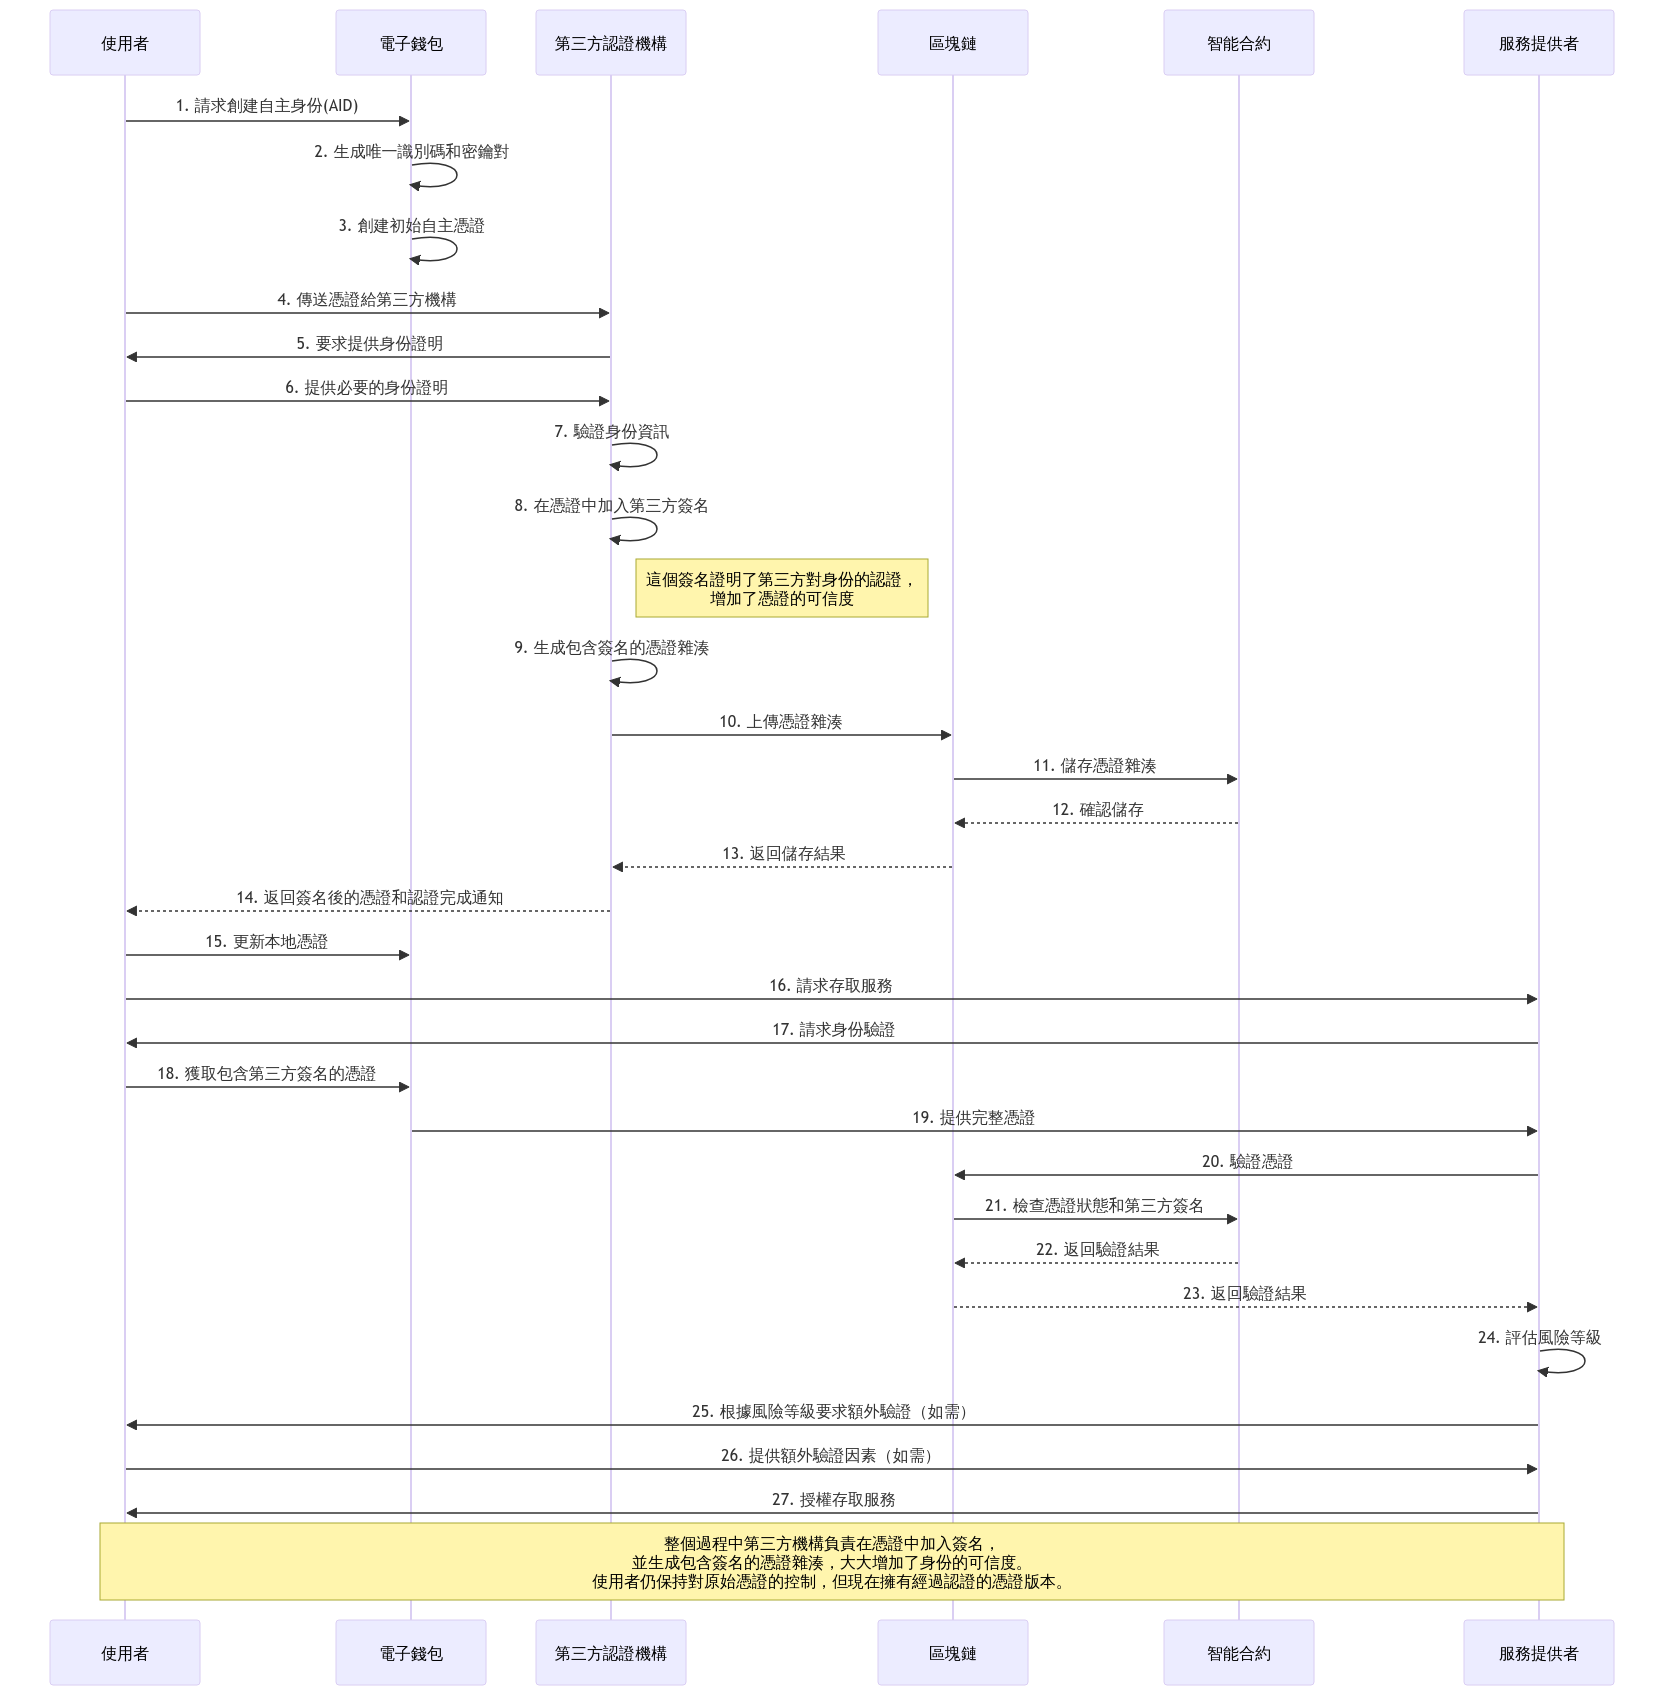
\includegraphics[width=\linewidth]{figures/full-aid-auth.png}
  \caption{AID系統完整自主驗證流程}
  \label{fig:appendix-full-aid-auth}
\end{figure}
\clearpage
\begin{figure}[p]
  \centering
  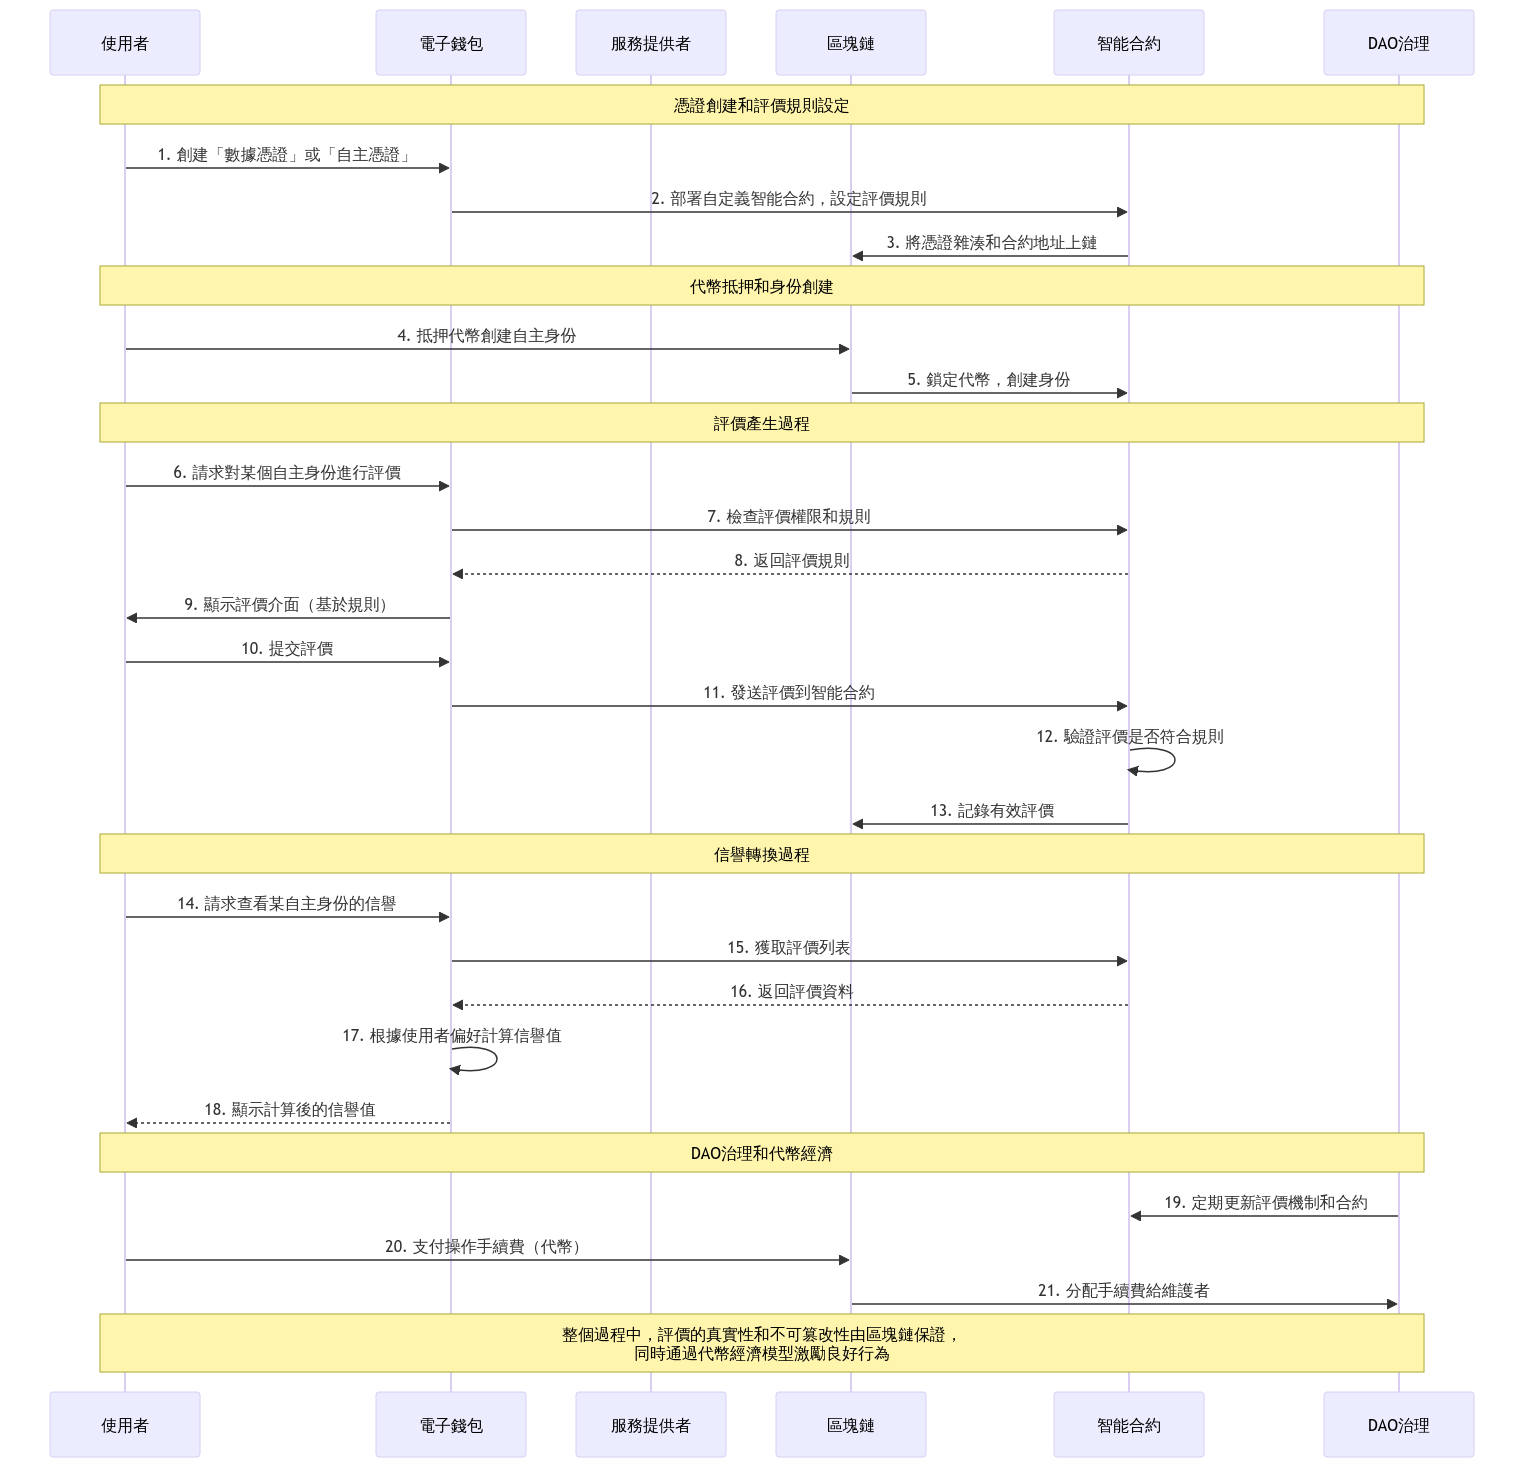
\includegraphics[width=\linewidth]{figures/credit-uml.png}
  \caption{信用評分流程}
  \label{fig:appendix-credit-uml}
\end{figure}
\section{流程圖}
流程圖詳細展示了AID系統中的特定流程,如多因素驗證和基於時空的分析,有助於理解系統的決策邏輯和操作步驟。
\begin{itemize}
  \item 圖 \ref{fig:appendix-emfa} 描述了極限多因素驗證的流程,展示了系統如何根據不同的風險級別要求不同程度的身份驗證。
  \item 圖 \ref{fig:appendix-time-space-analysis} 展示了基於時空的分析流程,說明了系統如何利用用戶的時間和空間信息來增強身份驗證的準確性。
\end{itemize}
\begin{figure}[p]
  \centering
  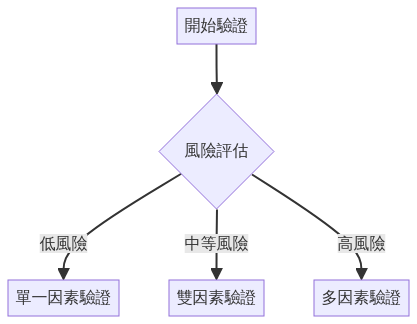
\includegraphics[width=\linewidth]{figures/EMFA.png}
  \caption{極限多因素驗證流程}
  \label{fig:appendix-emfa}
\end{figure}
\clearpage
\begin{figure}[p]
  \centering
  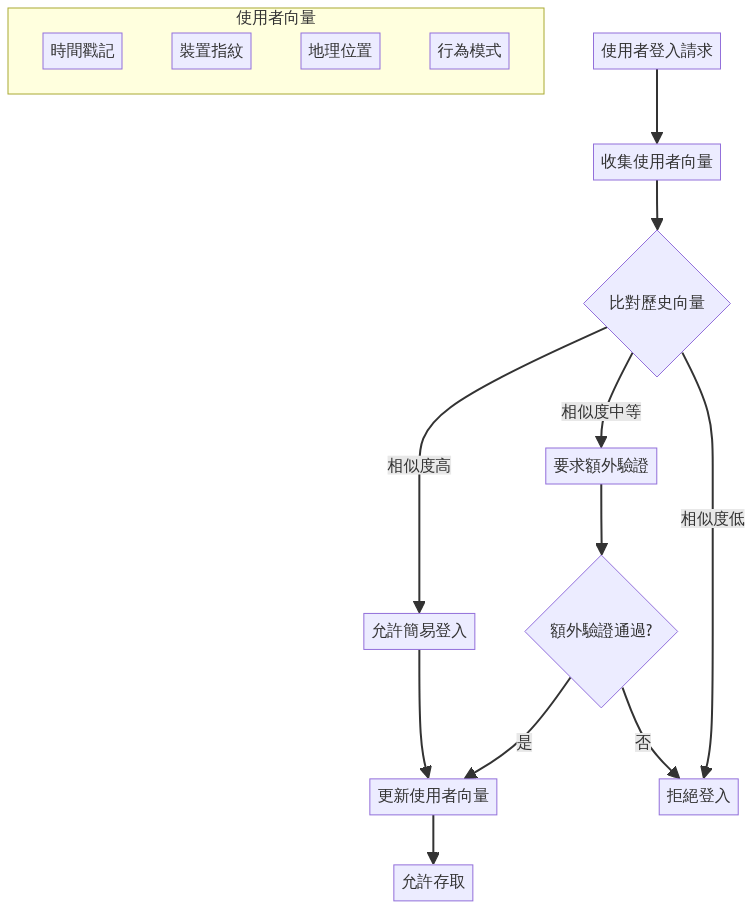
\includegraphics[width=\linewidth]{figures/time-space-analysis-uml.png}
  \caption{基於時空的分析流程}
  \label{fig:appendix-time-space-analysis}
\end{figure}